Producing a dataset suitable for analysis involves the workflow specified in \ref{analysis-workflow}. The workflow involves configuration of \textit{nETL} tasks to load data from CSVs into CouchDB, authoring of a CouchDB design doc, including a view function (MapReduce) and a list function, asking CouchDB to build the index, retrieving the indexed result via the list function specified in the design document and working with the joined dataset in Excel.

Analyses are conducted in an iterative fashion; with each iteration an increasing volume of data is handled so as to gain insight into the viability of handling varying amounts of data in CouchDB. Data volume is controlled by the number of courses analyses (more courses taken into account results in higher volumes of data), And the number of entities joined together (grades \& FU data vs grades, FU data, \& Sakai usage). Results are discussed in terms of the insights into business domain (EDM) as well as the effectiveness of the data-mining approach. Runtime results of \textit{nETL}, CouchDB indexing times, database/index storage footprints are shown in Table \ref{performance-analysis}.

\begin{figure}[ht]
    \centering
    \begin{mdframed}
        \centering
        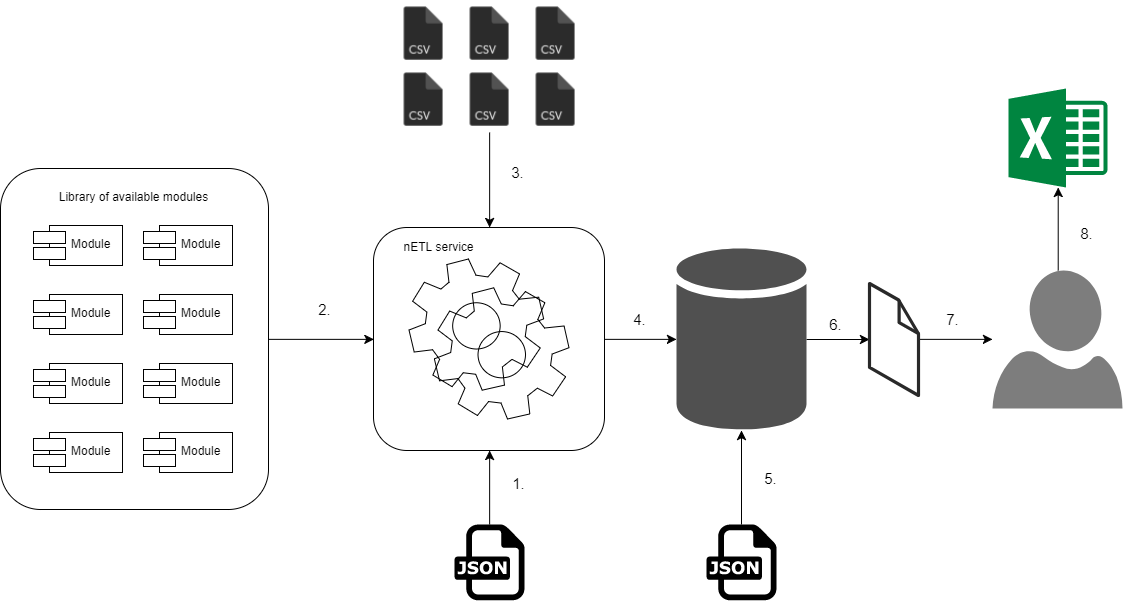
\includegraphics[scale=0.35]{./resources/figures/analysis-workflow.png}
    \end{mdframed}
    \caption[Analysis Workflow]{\textbf{Figure \ref{analysis-workflow}: Workflow to perform an analysis.}1) User creates a configuration file (JSON) that is loaded into the running \textit{\_nETL} service. This configuration includes instructions on which CSVs to load, which modules should be loaded to process the CSVs, and configurations for the modules. 2) Modules are loaded from a library of available modules into the \textit{\_nETL} service. 3) CSVs are loaded into the service, and transformations are applied to the CSV data as specified by the configuration in (1). 4) Data from the CSVs is loaded into CouchDB; this is also achieved via a module specified in (1). 5) A user creates a CouchDB design document, specifying the MapReduce functions, and a List function. 6) The user asks CouchDB to produce the view index as specified by the design document in (5). 7) The user retrieves the data from the view index using the list function specified in (5). 8) The user then loads the resultant CSV into Excel to produce useful metrics.}
    \label{analysis-workflow}
\end{figure}





\begin{table}[h]
    \begin{threeparttable}
        \textbf{Table \ref{performance-analysis}}\par\medskip\par\medskip
        \caption[Software performance analysis]{Running time analysis of \textit{nETL} tasks and CouchDB MapReduce indexing}
        \label{performance-analysis}
        \begin{tabularx}{\textwidth}{>{\hsize=1\hsize}Y>{\hsize=1\hsize}X>{\hsize=1\hsize}X>{\hsize=1\hsize}X>{\hsize=1\hsize}X}
            \toprule
            \mC{c}{}                                               & \mC{c}{Run 1} & \mC{c}{Run 2} & \mC{c}{Run 3} & \mC{c}{Run 4} \\
            \midrule
            Demographic lines extracted                            & 12 219        & 12 219        & 12 219        &               \\
            Demographic lines loaded                               & 1 381         & 9 874         & 595           &               \\
            Demographic task time (sec)\tnote{\textsuperscript{1}} & 2.488         & 3.114         & 6.755         &               \\
            Grade lines extracted                                  & 513 872       & 513 872       & 513 872       &               \\
            Grade lines loaded                                     & 1 891         & 79 849        & 738           &               \\
            Grade task time (sec)\tnote{\textsuperscript{1}}       & 37.684        & 42.001        & 97.221        &               \\
            Events lines extracted                                 & -             & -             & 44 420 508    &               \\
            Events lines loaded                                    & -             & -             & 661 555       &               \\
            Events task time (sec)\tnote{\textsuperscript{1}}      & -             & -             & 2 225.44      &               \\
            CouchDB footprint (MB)\tnote{\textsuperscript{2}}      & 0.9           & 23.2          & 172.1         &               \\
            View calculation time (sec)\tnote{\textsuperscript{3}} & 0.685         & 49.042        & 340.413       &               \\
            View size (MB)                                         & 0.813         & 143           & 521           &               \\
            \bottomrule
        \end{tabularx}
        \scriptsize
        \begin{tablenotes}
            \item[\textsuperscript{1}]Tasks are run asynchronously, so time taken includes processing of other tasks in this run. Task run times are printed out to the log
            \item[\textsuperscript{2}]This is representative of the amount of data processed by \textit{nETL}
            \item[\textsuperscript{3}]CouchDB views are calculated per shard. By default a database contains 8 shards (even in single node mode). The log file shows start and end times of view calculations for each shard, the time is taken as time the first shard starts indexing, to the time the last shard stops indexing.
        \end{tablenotes}
    \end{threeparttable}
\end{table}

